\chapter{Introduction}
\label{ch:intro}

Small devices increasingly have to recognise categories they were never trained on, often from one
to five labelled photos per new category. A practical way to do this is to take a network pretrained on
a large dataset, freeze it, and train only a small add-on module, an \emph{adapter}. Such adapters are
usually evaluated by one number, accuracy. This thesis asks what happens to the other parts of
reliability, namely whether the model's confidence can be trusted and whether it notices inputs that do
not belong to any known class, and which design choices control each of them.

\Cref{tab:headline} previews the answer. Each reliability aspect turned out to be controlled by a
different design choice, so no single choice makes the model reliable on every axis.

\begin{table}[H]
\centering
\caption{Which design choice governs which reliability aspect (details in \cref{ch:results}).}
\label{tab:headline}
\begin{adjustbox}{max width=\textwidth}
\begin{tabular}{@{}ll@{}}
\toprule
Reliability aspect & Governed mainly by \\
\midrule
Accuracy & shot count, then adapter architecture \\
Calibration & head type, then backbone \\
OOD detection & the uncertainty scoring rule \\
Repairing evidential calibration & a two-parameter post-hoc refit helps, but does not fully fix it \\
\bottomrule
\end{tabular}
\end{adjustbox}
\end{table}

\section{Background and Motivation}

Convolutional networks pretrained on ImageNet~\cite{deng2009imagenet} learn features that transfer
well to new visual tasks. The usual way to reuse them is full fine-tuning, which updates every weight.
When the new task has only a handful of labelled images per class, this is risky: a model with millions
of free parameters can fit five images in many ways, most of which do not generalise. This is the
setting of few-shot learning, where a model sees $K$ labelled examples per class (usually $K \in
\{1,5\}$) and must then classify new images of those classes~\cite{vinyals2016matching}.

Parameter-efficient fine-tuning (PEFT) keeps the pretrained network frozen and trains a small number of
new parameters instead. Bottleneck adapters~\cite{houlsby2019adapters} and low-rank adaptation
(LoRA)~\cite{hu2022lora} can approach the accuracy of full fine-tuning while training a tiny fraction of
the weights. Most of this work, however, targets large transformers on data-rich benchmarks. Lightweight
CNNs remain the practical choice for many edge devices~\cite{somvanshi2025tinydl}, and how adapters
behave inside them under few-shot scarcity has received much less attention.

Accuracy is also only one part of reliability. A model that says it is 95\% sure while being right
60\% of the time is \emph{miscalibrated}, and modern networks are known to be overconfident in this
way~\cite{guo2017calibration}. A related requirement is \emph{out-of-distribution (OOD) detection}:
recognising that an input belongs to none of the known classes instead of confidently assigning it to
one of them~\cite{hendrycks2017baseline}. Evidential deep learning (EDL)~\cite{sensoy2018edl} offers one
way to express this kind of uncertainty: the network outputs evidence for each class, which defines a
Dirichlet distribution, and a low total amount of evidence signals ``I don't know'' in a single forward
pass.

This thesis brings these threads together. We adapt frozen lightweight CNNs with small adapters, read
the output either as a softmax or as evidential evidence, and measure accuracy, calibration and OOD
detection on the same trained models.

\section{Problem Statement}

The study starts from one observation: a model can be accurate and still unreliable.
\Cref{fig:reliability} shows the two failure modes we measure. On the left, a known-class input is
misclassified with high confidence; on the right, an input from an unseen class is confidently assigned
to a known class. Neither failure shows up in an accuracy number.

\begin{figure}[H]
\centering
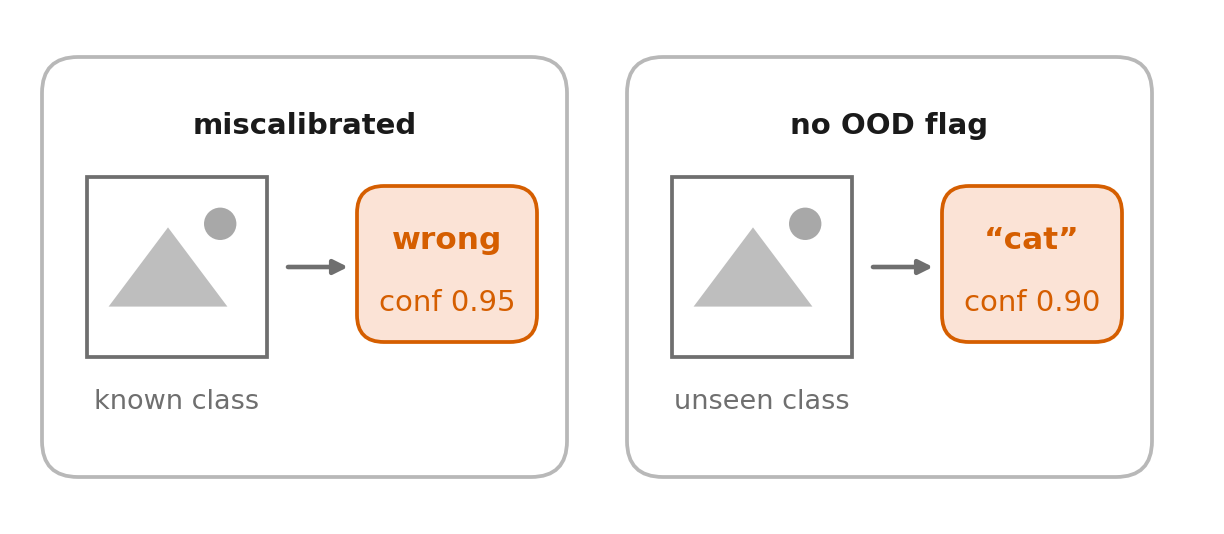
\includegraphics[width=0.85\textwidth]{D1_accuracy_vs_reliability.png}
\caption{Accuracy is not reliability. Left: a known-class input confidently misclassified
(miscalibration). Right: an input from an unseen class confidently assigned to a known class (no OOD
flag).}
\label{fig:reliability}
\end{figure}

Three gaps motivate the work:
\begin{itemize}
\item \textbf{Full fine-tuning is expensive and fragile in the few-shot regime.} It updates millions of
weights from a few images per class and must be stored per task.
\item \textbf{PEFT studies rarely measure reliability.} Adapter papers usually report accuracy only, so
it is unclear what an adapter does to confidence and OOD behaviour.
\item \textbf{PEFT research focuses on transformers.} Adapters, LoRA and prompt tuning were developed
for and mostly evaluated on transformers~\cite{houlsby2019adapters,hu2022lora,jia2022vpt,chen2022adaptformer}.
CNN-side work exists~\cite{chen2024convadapter,li2022tsa,aleem2024convlora,zhong2024convlora} but rarely
combines PEFT with calibration and OOD evaluation.
\end{itemize}

\Cref{tab:challenges} pairs each gap with the design decision we take in response. This is an
evaluation study, not a new model: we use existing adapters and heads and compare them under one
controlled protocol.

\begin{table}[H]
\centering
\caption{The three gaps and how this thesis responds to each.}
\label{tab:challenges}
\begin{tabularx}{\textwidth}{@{}>{\raggedright\arraybackslash}p{5.2cm}X@{}}
\toprule
Gap & Our response \\
\midrule
Full fine-tuning updates millions of weights & Freeze the backbone and train at most 31.7K adapter
parameters once. New classes need no further gradient steps. \\
PEFT studies rarely measure reliability & Measure accuracy, calibration and OOD detection on the same
runs. \\
PEFT research focuses on transformers & Study adapters inside frozen lightweight CNNs. \\
\bottomrule
\end{tabularx}
\end{table}

\section{Research Questions}

Published comparisons in this area often change two things at once, for example the training objective
and the uncertainty score, or the adapter's design and its size. We therefore ask questions about
\emph{what governs} each outcome rather than which single model is best:

\begin{description}[leftmargin=1.2cm,style=nextline]
\item[RQ1] Which design choices most strongly explain variation in accuracy, calibration and OOD
detection? That is, how is the variance of each outcome distributed across dataset, shot count,
backbone, adapter type and head?
\item[RQ2] Is OOD detection explained more by the training objective (evidential or softmax) or by the
scoring rule used to read the model's outputs (MSP, temperature-scaled MSP, energy or vacuity)?
\item[RQ3] Does accuracy follow adapter architecture, and calibration follow the trainable-parameter
budget, or does something else decide calibration?
\item[RQ4] Can the calibration of the evidential head be repaired after training, by refitting only its
two evidence parameters on validation episodes, without breaking its OOD ranking?
\end{description}

\Cref{tab:rqs} lists the evidence each question is answered with, and \cref{fig:roadmap} shows how the
four fit under one overall question.

\begin{table}[H]
\centering
\caption{The four research questions and the evidence used to answer them.}
\label{tab:rqs}
\begin{tabularx}{\textwidth}{@{}lXl@{}}
\toprule
& Question & Answered by \\
\midrule
RQ1 & Which design choices explain accuracy, calibration and OOD detection? & 120-run factorial grid \\
RQ2 & Training objective or scoring rule for OOD detection? & all 120 models re-scored 4 ways \\
RQ3 & Does accuracy follow architecture and calibration follow budget? & grid + matched-budget experiment \\
RQ4 & Can evidential calibration be repaired post hoc? & refit of 60 evidential models \\
\bottomrule
\end{tabularx}
\end{table}

\begin{figure}[H]
\centering
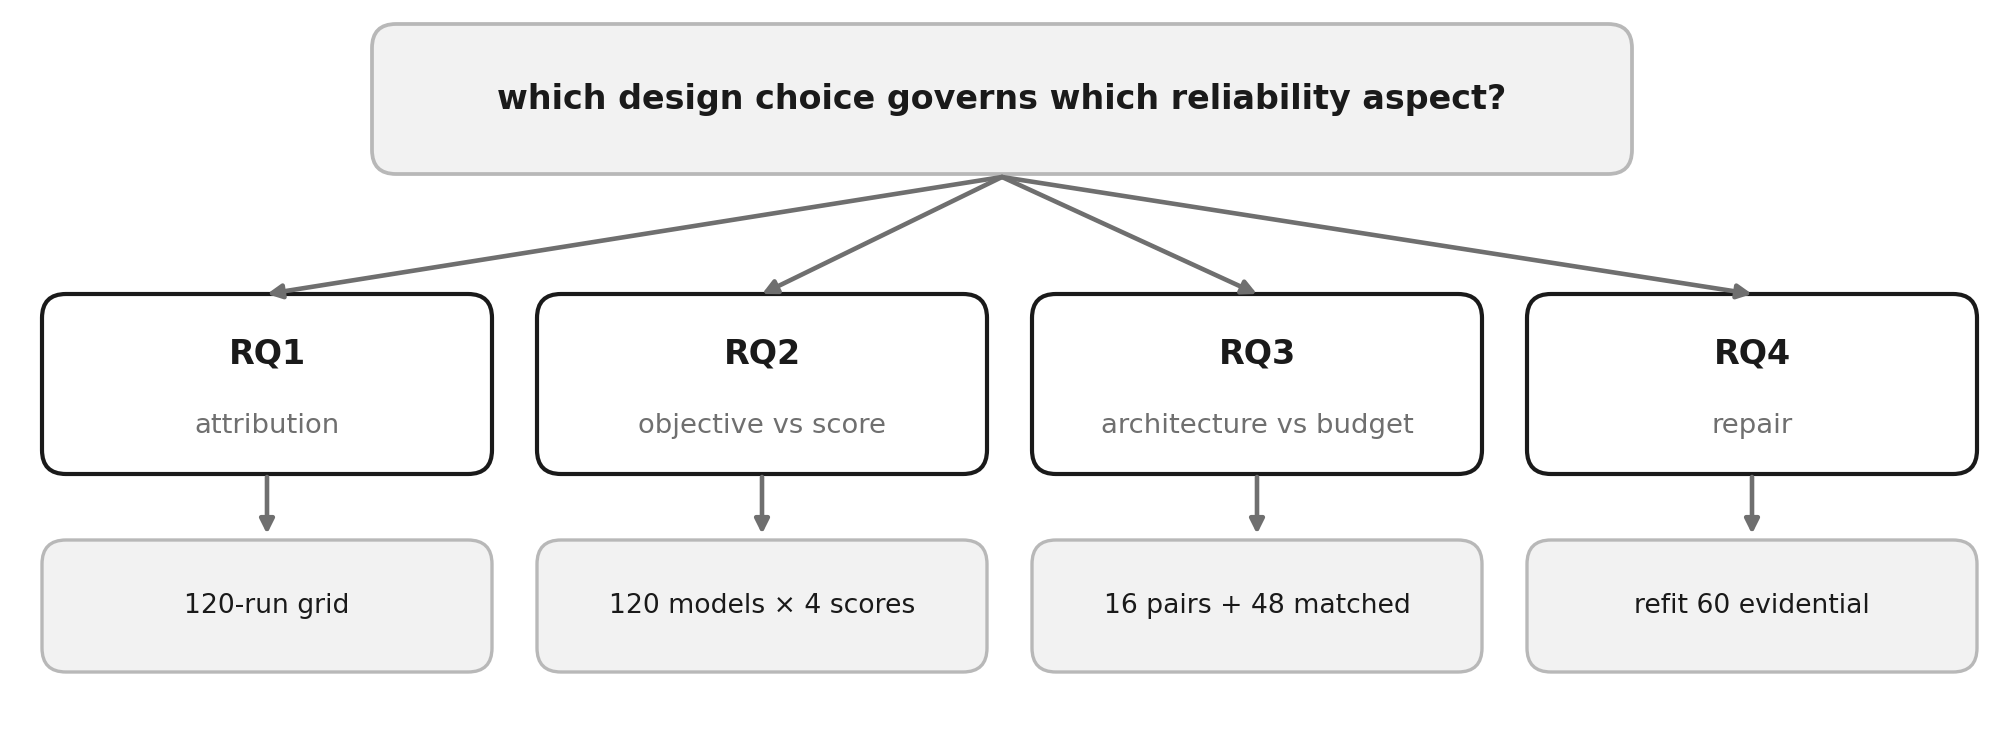
\includegraphics[width=0.95\textwidth]{F1_research_roadmap.png}
\caption{The four research questions are instances of one question: which design choice governs which
reliability aspect.}
\label{fig:roadmap}
\end{figure}

\section{Research Challenges}

\paragraph{Confounded comparisons.} Two adapters rarely differ in one property only. In our grid the
bottleneck adapter is the larger adapter on ResNet-18 but the smaller one on MobileNetV3-Small, so
adapter size and backbone always change together. Separating them required a dedicated matched-budget
experiment (\cref{sec:rq3}).

\paragraph{A fragile evidential head.} Our first evidential model did not train at all. Softplus was
applied directly to negative squared-distance logits of magnitude in the hundreds, so every class
received essentially zero evidence and the gradients vanished. Switching to scaled cosine logits and
adding a learnable scale and bias before the softplus (\cref{sec:readouts}) fixed this, and those two
parameters later became the subject of RQ4.

\paragraph{Noisy few-shot estimates.} With one or five support images, a single episode says little.
Every number in this thesis is averaged over the same 600 fixed test episodes and over three training
seeds.

\section{Contributions}

\begin{enumerate}
\item \textbf{A controlled, reliability-complete comparison.} A balanced 120-run grid (40
configurations $\times$ 3 seeds) of frozen lightweight CNNs with small adapters, evaluated for accuracy,
macro-F1, calibration (ECE, Brier) and OOD detection (AUROC, FPR@95) on the same 600 test episodes.
\item \textbf{A variance decomposition (RQ1).} Shot count explains about 76\% of accuracy variance and
head type about 83\% of calibration variance, while the head explains only 0.2\% of accuracy variance.
\item \textbf{A separation of training objective from scoring rule (RQ2).} Scoring every model with
every score shows that the score explains 42.7\% of far-OOD variance against 0.17\% for the objective.
The energy score works almost as well on evidential-trained logits as on softmax-trained ones.
\item \textbf{A pre-registered matched-budget experiment (RQ3).} At equal parameter budget, accuracy and
near-OOD detection still follow adapter architecture, whereas the calibration gap follows the backbone
rather than the budget.
\item \textbf{A measured post-hoc repair (RQ4).} Refitting two parameters improves evidential
calibration in 60 of 60 models; we report both what it repairs and what it costs in OOD ranking.
\end{enumerate}

\section{Thesis Organization}

\Cref{ch:related} reviews related work and positions the thesis. \Cref{ch:data} describes the datasets,
backbones, episodic protocol and metrics. \Cref{ch:method} describes the system and the experimental
design. \Cref{ch:results} answers the four research questions and discusses deployment cost,
positioning and limitations. \Cref{ch:conclusion} concludes. \Cref{app:tables} contains the full result
tables.
